\chapter[Snake]{Habitat dimensionality and a diet of eggs: The evolution of venom loss in snakes.}
\label{chap:Snake}



\begin{figure}[h]

  \includegraphics[width=.5 \textwidth, right]{ch4-snakes/venom.png}
\end{figure}


\begin{quoteshrink}
  ``Always keep your smile. That's how I explain my long life.''
  
\hfill{Jeanne Calment}
\end{quoteshrink}

\begin{abstract}

The evolution of venom in snakes offers a system of ecological, evolutionary and medical interest. Despite this many fundamental questions regarding the evolution and variation of this trait amongst snakes still persist, such as the perplexing range in the toxicity and quantities venom across species. For example despite the obvious benefits of possessing venom many species have secondarily either lost or severely reduced the toxicity or volume of venom produced. One of the potential answers to this paradox is the reduction of costs associated with producing large amounts of venom in species were the benefits of venom are reduced. Here I test several hypothesis on such ecological factors that may be associated with the atrophy of venom in snakes including habitat dimensionality, which is predicted to affect encounter rates, diet and body size. Further to this I test the co-evolutionary relationship between venom toxicity and venom volume along with the levels of prey-specificity in a comparative analysis using over 100 species of venomous snakes. I find that species with associations to high dimensional habitats and a diet of eggs show atrophy of venom through reduced venom volumes and in the case of eggs eating reduced toxicity. These results also show that, despite predictions, levels of toxicity show no association with the volume of venom produced. However snake venom was found to be prey-specific with venoms tested on models closely related to the diets of that species showing higher levels of toxicity. Overall snake venom provides a remarkable case of predator-prey interactions with a rapidly shifting arms race dynamic. Understanding venom evolution is hence both important to our understating of predator trait evolution as a whole and the ecology of this important predatory group.


\end{abstract}

\section{Introduction}

The evolution of predatory traits can often be the defining feature of whole clades of animals, from the evolution of the first jawed fish to the use of silk for web construction in arachnids. Perhaps nowhere is this better illustrated then in the evolution of venom in snakes. Through the processes of limb reduction and eventual loss beginning over 160 million years ago \citep{caldwell2015oldest} snakes have relied on extreme adaptations in order to capture and kill prey items such as complex cocktails of venoms \citep{casewell2013complex,fry2012structural}. This reliance on venom as a primary means to capture prey in many species of snakes makes them an excellent group to study how fundamental aspects of ecology, such as habitat dimensionality, can drive the evolution of predatory traits and predator-prey interactions.


Venoms, which can be broadly defined as "a secretion produced in a specialised gland in one animal and delivered to a target animal through the infliction of a wound, which contains molecules that disrupt normal physiological or biochemical process so as to facilitate feeding or defence by the producing animal" \citep{casewell2013complex}, in snakes consist of complex cocktails of proteins and other compounds creating neurotoxic and hemotoxic compounds \citep{greene1997snakes,casewell2013complex}. While the biological properties these mixtures possess has lead to a wide body of biomedical research there is surprising little understanding of the ecological pressures associated with the evolution of the diverse venoms found in snakes \citep{greene1997snakes,casewell2013complex}. Functionally venoms are used for both foraging and anti-predator defence. However anti-predatory defence is likely to be secondary functionality of venoms, as reflected by the lack of correlation between lifespan and the possession of venom in snakes \citep{hossie2013species}, with aiding in prey acquisition a more likely primary function (ref). However despite the clear functionality and benefits associated with possessing venom many species of snakes have paradoxically lost this ability secondarily. Such atrophy of venom toxicity, production and of the apparatus required to deliver venom is seen at the most extreme vestigial state in the sea snake \textit{Aipysurus eydouxii} \citep{li2005eggs}, but is also seen as various levels of atrophy of toxicities or venom volumes produced in other species \citep{fry2012structural}. One possible solution to this paradox is the investment cost associated with the production of venoms.


Venom synthesis carries an appreciable cost both with regards to energy requirements and through possible lost opportunities. After venom extraction pitvipers have been shown to greatly increase their metabolic rates over a 72 hour periods \cite{mccue2006cost}, and while other species indicate less severe costs \citep{pintor2010costs}, species that heavily dependent on their venom to capture prey would undergo lost opportunities over the replenishment period. This cost is reflected in the behaviours of some rattlesnake species that meter the amount of venom they inject into their prey species \citep{hayes1995venom} and also through the occurrence of dry bites associated with defensive behaviour \citep{morgenstern2013venom}. This cost of venom explains the loss or reduction of venom in many species, for example a switch to a diet of eggs in \textit{Aipysurus eydouxii} is likely to be the driver of venom loss in this species due to the removal of the need to incapacitate their prey. However many species of similar size and diet still show considerable variation in the toxicity and volume of venom they produce pointing towards other ecological or evolutionary drivers of venom evolution.



One key component in the evolution of venom is the identity of the target prey species. The venoms of several species of snake show a strong prey-specific element with regards to the toxicity. For example \cite{barlow2009coevolution} showed that within \textit{Echis} viper populations that feed on different prey groups, individuals show higher toxicities for their preferred prey items. Similarly Malaysian pit vipers show variation in their venoms that correlate with diet \citep{daltry1996diet}. However such prey-specificity in venom does not seem to be present in all snakes species making the ubiquity of this interaction unclear \citep{williams1988variation}. One possible explanation for this is the arms race between the evolution of venom potency in snakes and the corresponding evolution of resistance in species under heavy predation, such as ground squirrels showing resistance to their rattlesnake predators \citep{poran1987resistance}. In fact there is some evidence that such resistance to pitviper venoms in Opossums has led to a switch in predator-prey roles with Opossums now the predators of pitvipers \citep{voss2013opossums}. This arms race has resulted in the rapid evolution of genes associated with venom as demonstrated in the king cobra genome \citep{vonk2013king}, however a simpler evolutionary response to such resistance may be to increase the amount of venom a species produces.


The evolution of snake toxicity depends on rapid genomic evolution, such as through gene duplication events, in order to stay apace with prey resistance \citep{vonk2013king}. Such evolutionary events are likely to be relatively rare which may result in species relying on increased venom doses in order to keep pace with short term prey resistance responses. Species which show low toxicities would hence be expected to compensate by producing larger reservoirs of venom with which to increase dosages to prey while species with high toxicities would be expected to reduce venom production in order to offset unnecessary costs \citep{mccue2006cost}. Such variation in prey resistance may also lead to "overkill" type behaviours were individuals inoculate doses far in excess of that required to incapacitate prey items (ref). This overkill behaviour is also likely to in part be an artefact to the common use of mice to determine venom toxicities instead of a snakes natural prey. A more realistic interpretation of the data requires including the physiological distance such test species may have in comparison to snakes diet. Overall a correlation between venom toxicity and volume would be expected if snakes use compensatory behaviour while species with a diet close to that of the test model would be expected to show higher toxicities indicative of adaptive prey specific venoms. While the evolution of venom is likely to be strongly influenced by the arms race between predator and prey, the ability to simply find a prey item may also be an important determinant in the volume and toxicity of a snakes venom.


While incapacitating prey is primary function of venom, venom evolution might also be expected to be influenced by the probability of encountering such a prey item. One such aspect which may influence these probabilities is habitat dimensionality \citep{pawar2012dimensionality} as encounter rates show higher scaling with body mass in higher dimensional environments. This may decrease the investment in venom production due to the higher probability of encountering prey reducing lost opportunities of missed strikes or though the faster replenishment rates in order to fully exploit such encounters, which may be associated with the faster digestion rates seen in arboreal species \citep{lillywhite2002patterns}. Conversely high habitat dimensionality may also increase the venom volume produced through the increased capacity of prey species to escape in multiple directions or selection to higher toxicities \citep{healy2014ecology,moller2010up}. 


Here I use a comparative approach in order to test multiple hypothesis on venom evolution in snakes. Using data on venom toxicity, volume produced, size, diet and environment I test using a multiple response model the relationship between venom toxicity using median lethal dose as a measure and both maximum and mean venom volumes found in snakes. I also test whether species that have diets photogenically similar to the test animal used to determine toxicity show increased toxicities and whether species that include eggs within their diet show atrophy of both venom toxicity and volume. Finally I test whether species that inhabit high dimensional environments, namely arboreal and aquatic species, show differences in the venom volume and toxicity. Overall I find that species in high dimensional habitats or that consume eggs show a reduction in both maximum and mean venom volumes produced and also that snakes show higher toxicities to species that are physioligically closer to that found within their diet.

\section{Materials and Methods}
\subsection{Data}

As a measure of venom toxicity I used median lethal dose (LD$_{50}$), the individual dose required to kill 50\% of a population of test animals, were lower values of LD$_{50}$ indicate a higher venom toxicity. As the route of inoculation can affect LD$_{50}$ (ref) only values estimated from either intravenous, subcutaneous, intrapulmonary or intramuscular inoculation routes were used, with a fixed term included to account for the variation between these routes. While most studies determine LD$_{50}$ values using murine test animals I also included studies that used alternative models as snake venom potency is likely to be linked to diet \citep{barlow2009coevolution}. I used both reported maximum and mean dry weight (mg) as a measure of venom volume as the dry weight represents the active proteinaceous component of venom and as it was the most available reported measure. In the case of multiple studies reported venom volumes the mean values across the studies were taken as the value for that species with the maximum across all studies used as the overall maximum value.


Diet data was collated from the literature using studies with quantitative estimates of prey proportions, mainly from studies of stomach contents (See appendix for data). As prey items were rarely identified to lower taxonomic levels diet was categorized as in \citep{allen2013evolution} into six prey categories; invertebrates, fish, amphibians, lizards, birds and mammals. A separate term indicating the inclusion of eggs within a species diet was also included.


To test whether snakes with prey phylogenetically close to the LD$_{50}$ test had higher toxicities I calculated a score relating to the phylogenetic distance between the test species used to calculate the LD$_{50}$ value and the groups present in the snakes diet. This was calculated as the sum of the phylogenetic distance, using average estimates from TimeTree \citep{hedges2006timetree}, between each prey group and the LD$_{50}$ model by the proportion of each prey group reported in each snake species diet. For example a species with a diet of 20\% mammals, 50\% fish and 30\% reptiles with a LD$_{50}$ measured using mice would have a score of 0.2\*(0) + 0.5\*(400.1) + 0.3\*(296) = 288.85.


Species habitat was categorised as either terrestrial, fossorial, aquatic or arboreal based on literature accounts. In order to directly test any effect of the dimensionality of habitat environment each environment was scored, as in \citep{pawar2012dimensionality}, with terrestrial and fossorial environments scored as two-dimensional and arboreal and aquatic scored as three-dimensional.
As venom volume is known to increase with body size \citep{mirtschin2002influences}, it was included in the analysis using total length values from the literature, primarily from the compilation of \citep{boback2003empirical} and from field guides and other works on regional snake faunas. To allow direct comparison with other allometric scaling studies body length was converted into mass using the conversion in \citep{boback2003empirical}. 


Mass, LD$_{50}$, venom volume and phylogenetic distance between diet and model were log10 transformed, mean centred and expressed in units of standard deviation prior to analysis. Significance was determined for the fixed effects when 95\% of the data is greater or less than 0. To correct for phylogeny I used the tree from (\cite{pyron2014early}, Figure 1). 


\begin{figure}[h]
  \centering
  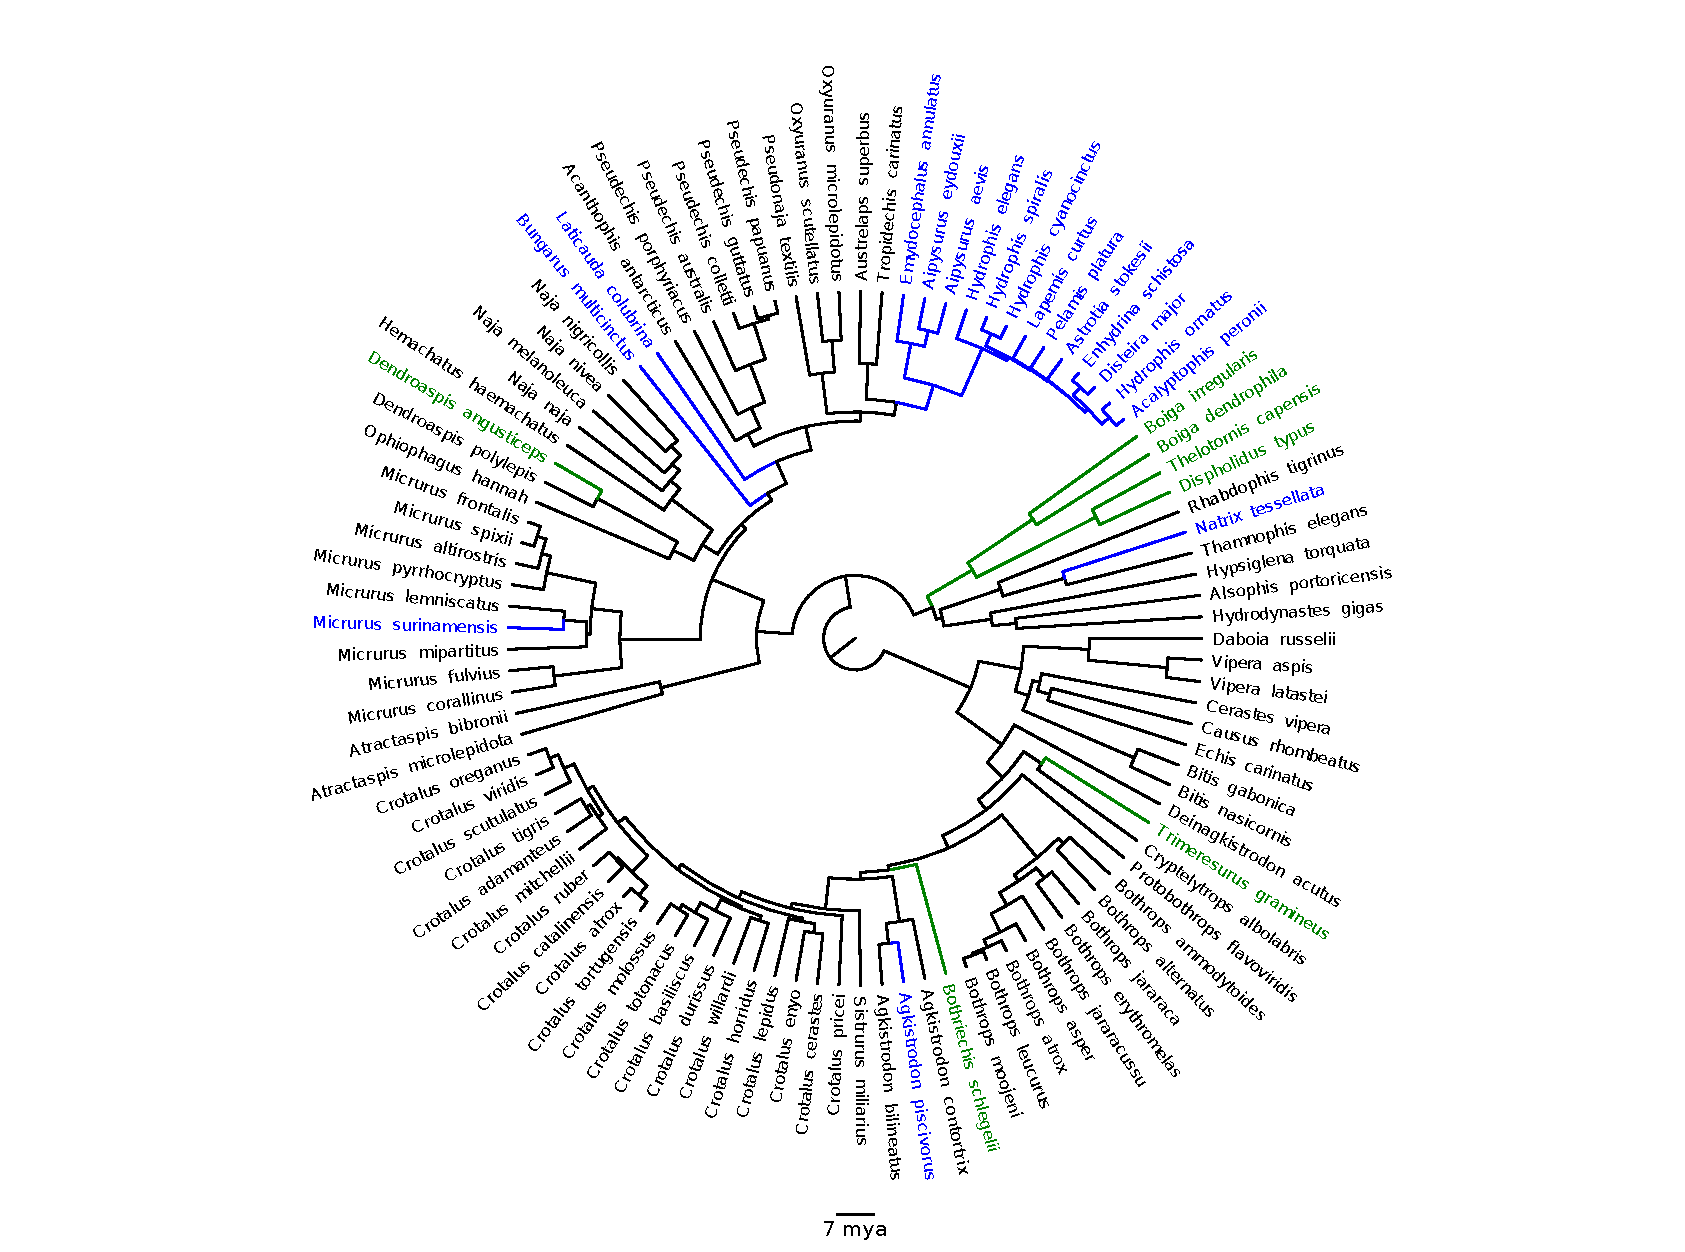
\includegraphics[width=.95\textwidth]{ch4-snakes/fig1_snake_phylo.pdf}%Note that this is the path for the folder
  %for chapter 2 that has the Tastes_funny.jpg file within it.
  \caption[Figure 1.]{Phylogeny}
  \label{fig:Figure 1.}
\end{figure}


Overall data was collated for 101 species (76 species with maximum venom volume estimates, 99 species with average venom volume estimates).


\subsection{Analyses}

To test these hypotheses I fit multiple response phylogenetic mixed models using the MCMCglmm package \citep{hadfield2010mcmc} in R 2.14.2 \citep{RCran}. As venom volume and LD$_{50}$ are likely to have co-evolved both were included as response variables with mass, LD$_{50}$ inoculation method, habitat dimensionality, the presence of eggs in diet and phylogenetic distance from LD$_{50}$ model included as explanatory variables. I fit two separate models; one using maximum venom volume and one with average venom volume. Phylogeny was controlled by including it using the animal term in the MCMCglmm model \citep{hadfield2010mcmc}. Variation due to multiple measures on individual species, mostly to allow the inclusion of separate values for sub-species, was included using a separate random term at the species level. All models were fitted with uninformative priors by using inverse-Wishart parameter expanded priors \citep{hadfield2010mcmc} with burn-in, thinning and number of iterations determined to ensure effective sample sizes exceeded 1000 for all parameter estimates and convergence tested using the Gelman-Rubin statistic \citep{gelman1992inference}. 

\section{Results}

After controlling phylogeny these analysis showed that smaller species that inhabit high dimensional environments have both lower mean and maximum volumes of venom (Figures 1 and 2, Tables 2 and 5). Toxicity was affected by the route of inoculation, with intravenous and intrapulmonary inoculation routes showing lower LD$_{50}$ in comparison to subcutaneous measures, and the phylogenetic distance between the LD$_{50}$ model and species diet, with diets closer to the LD$_{50}$ model showing higher toxicities (Tables 3 and 6). Species with egg based diets showed a reduction in toxicity and maximum venom volume but not average venom volume (Tables 2,3,5,6).




\begin{figure}[h!]
  \centering
  \includegraphics[width=.95\textwidth]{ch4-snakes/figure2aver.pdf}%Note that this is the path for the folder
  %for chapter 2 that has the Tastes_funny.jpg file within it.
  \caption[Figure 2a.]{Mean}
  \label{fig:Figure 1.}
\end{figure}




\begin{figure}[h!]
  \centering
  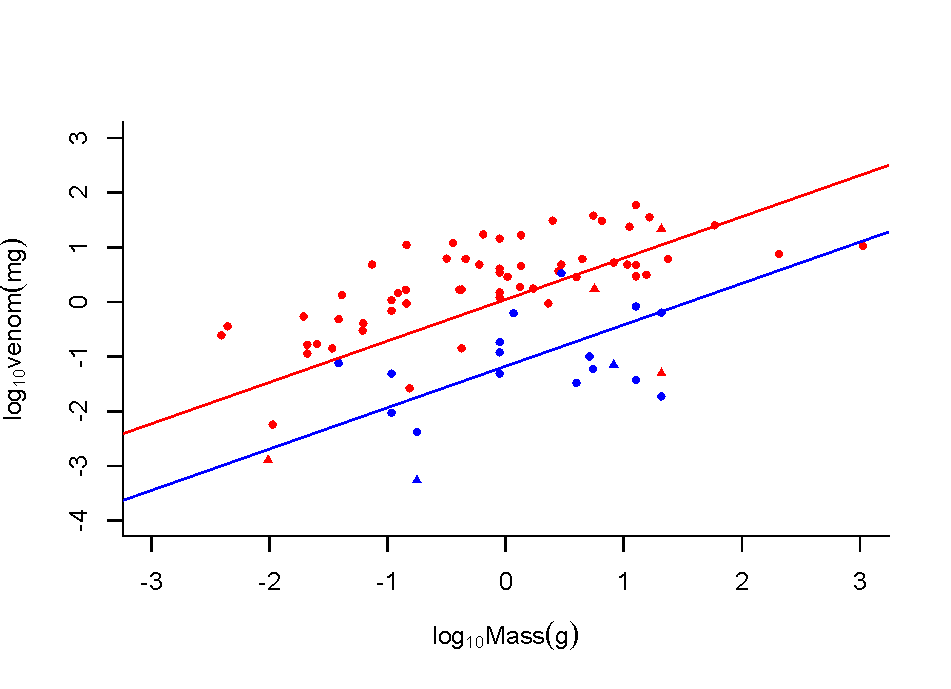
\includegraphics[width=.95\textwidth]{ch4-snakes/figure2max.pdf}%Note that this is the path for the folder
  %for chapter 2 that has the Tastes_funny.jpg file within it.
  \caption[Figure 2b.]{Max}
  \label{fig:Figure 2b.}
\end{figure}



Their was no correlation between LD$_{50}$ and either maximum or mean venom volumes (Tables 1 and 4). Both LD$_{50}$  and venom volume show high phylogenetic variance with phylogeny showing a higher association in LD$_{50}$ in comparison to venom volume in both models (Tables 1 and 4). 

\begin{table}[h!]
  \centering
    \caption[Table 1.]{Correlation structure on random terms.}
\begin{tabular}{*5l}    \toprule
\emph{Terms} & \emph{Estimate} & \emph{Lower CI} & \emph{Higher CI}\\\midrule
\textbf{Phylogeny} &   &   &  \\ 
Variance: Mean volume & 0.456 & 0.145 & 0.847 \\
Covariance: Mean volume and LD$_{50}$ & -0.003  & -0.290  & 0.301 \\
Variance: LD$_{50}$ & 0.909 & 0.479 & 1.452 \\

 &   &   &  \\

\textbf{Residuals} &   &   &  \\ 
Variance: Mean volume & 0.009 & 0.007 & 0.011 \\
Covariance: Mean volume and LD$_{50}$ & 0.003  & -0.004  & 0.011 \\
Variance: LD$_{50}$ & 0.268 & 0.215 & 0.328 \\

 &   &   &  \\ 

\textbf{Species} &   &   &  \\ 
Variance: Mean volume & 0.308 & 0.156 & 0.462 \\
Covariance: Mean volume and LD$_{50}$ & 0.030  & -0.040  & 0.118 \\
Variance: LD$_{50}$ & 0.055 & 0.001 & 0.170 \\\bottomrule
 \hline
\end{tabular}
  \label{tbl:Table 1.}
\end{table}




\begin{table}[h!]
  \centering
    \caption[Table 2.]{Volume in average volume.}
\begin{tabular}{*5l}    \toprule
\emph{Fixed Terms} & \emph{Estimate} & \emph{Lower CI} & \emph{Higher CI}\\\midrule
\textbf{Intercept} & 0.200  & -0.161 & 0.567 \\ 
\textbf{Body Mass} & 0.510  & 0.442 & 0.564 \\ 
\textbf{Inoculation Route} &  &  &  \\ 
 Intravenous (IV) & -0.011 & -0.052 & 0.030 \\
 Intrapulmonary (IP) & -0.010 & -0.052 & 0.030 \\ 
 Intramuscular (IM) & -0.009 & -0.056 & 0.042 \\
  &  &  &  \\ 
\textbf{Dimension 3D} & -0.829 & -1.286 & -0.396 \\ 
\textbf{Eggs in diet} & -0.741 & -1.325 & -0.206 \\ 
\textbf{Phylogenetic disparity of diet to model} & -0.003 & -0.029 & 0.019 \\\bottomrule
 \hline
\end{tabular}
  \label{tbl:Table 2.}
\end{table}



\begin{table}[h!]
  \centering
    \caption[Table 3.]{ld50 in average volume model}
\begin{tabular}{*5l}    \toprule
\emph{Fixed Terms} & \emph{Estimate} & \emph{Lower CI} & \emph{Higher CI}\\\midrule
\textbf{Intercept} & 0.200  & -0.161 & 0.567 \\ 
\textbf{Body Mass} & 0.134  & 0.016 & 0.262 \\ 
\textbf{Inoculation Route} &  &  &  \\ 
 Intravenous (IV) & -0.624 & -0.842 & -0.435 \\
 Intrapulmonary (IP) & -0.537 & -0.746 & -0.309 \\ 
 Intramuscular (IM) & -0.228 & -0.455 & 0.049 \\
  &  &  &  \\ 
\textbf{Dimension 3D} & -0.202 & -0.670 & 0.243 \\ 
\textbf{Eggs in diet} & 0.457 & -0.187 & 1.065 \\ 
\textbf{Phylogenetic disparity of diet to model} & 0.360 & 0.248 & 0.463 \\\bottomrule
 \hline
\end{tabular}
  \label{tbl:Table 3.}
\end{table}





%%%%%new set of tables

\begin{table}[h!]
  \centering
    \caption[Table 4.]{Correlation structure on random terms in maximum venom}
\begin{tabular}{*5l}    \toprule
\emph{Terms} & \emph{Estimate} & \emph{Lower CI} & \emph{Higher CI}\\\midrule
\textbf{Phylogeny} &   &   &  \\ 
Variance: Maximum volume & 0.500 & 0.156 & 0.960 \\
Covariance: Maximum volume and LD$_{50}$ & 0.156  & -0.181  & 0.496 \\
Variance: LD$_{50}$ & 0.901 & 0.349 & 1.477 \\

 &   &   &  \\

\textbf{Residuals} &   &   &  \\ 
Variance: Maximum volume & 0.003 & 0.002 & 0.004 \\
Covariance: Maximum volume and LD$_{50}$ & 0.006  & 0.001  & 0.012 \\
Variance: LD$_{50}$ & 0.275 & 0.001 & 0.361 \\

 &   &   &  \\ 

\textbf{Species} &   &   &  \\ 
Variance: Maximum volume & 0.230 & 0.103 & 0.373 \\
Covariance: Maximum volume and LD$_{50}$ & -0.036  & -0.141  & 0.052 \\
Variance: LD$_{50}$ & 0.061 & 0.001 & 0.188 \\\bottomrule
 \hline
\end{tabular}
  \label{tbl:Table 4.}
\end{table}


\begin{table}[h!]
  \centering
    \caption[Table 5.]{Volume in Maximum volume.}
\begin{tabular}{*5l}    \toprule
\emph{Fixed Terms} & \emph{Estimate} & \emph{Lower CI} & \emph{Higher CI}\\\midrule
\textbf{Intercept} & 0.043  & -0.339 & 0.379 \\ 
\textbf{Body Mass} & 0.757  & 0.708 & 0.797 \\ 
\textbf{Inoculation Route} &  &  &  \\ 
 Intravenous (IV) & -0.006 & -0.031 & 0.019 \\
 Intrapulmonary (IP) & 0.008 & -0.019 & 0.037 \\ 
 Intramuscular (IM) & 0.003 & -0.037 & 0.047 \\
  &  &  &  \\ 
\textbf{Dimension 3D} & -1.212 & -1.638 & -0.763 \\ 
\textbf{Eggs in diet} & -0.564 & -1.219 & 0.063 \\ 
\textbf{Phylogenetic disparity of diet to model} & -0.001 & -0.032 & 0.033 \\\bottomrule
 \hline
\end{tabular}
  \label{tbl:Table 5.}
\end{table}



\begin{table}[h!]
  \centering
    \caption[Table 6.]{ld50 in maximum volume model}
\begin{tabular}{*5l}    \toprule
\emph{Fixed Terms} & \emph{Estimate} & \emph{Lower CI} & \emph{Higher CI}\\\midrule
\textbf{Intercept} & 0.043  & -0.339 & 0.379 \\ 
\textbf{Body Mass} & 0.145  & -0.018 & 0.305 \\ 
\textbf{Inoculation Route} &  &  &  \\ 
 Intravenous (IV) & -0.656 & -0.892 & -0.440 \\
 Intrapulmonary (IP) & -0.561 & -0.804 & -0.326 \\ 
 Intramuscular (IM) & -0.191 & -0.531 & 0.152 \\
  &  &  &  \\ 
\textbf{Dimension 3D} & 0.240 & -0.300 & 0.836 \\ 
\textbf{Eggs in diet} & 0.705 & 0.076 & 1.510 \\ 
\textbf{Phylogenetic disparity of diet to model} & 0.251 & 0.080 & 0.436 \\\bottomrule
 \hline
\end{tabular}
  \label{tbl:Table 6.}
\end{table}




\section{Discussion}


These results show that, after controlling for body size and phylogeny, the evolution of venom in snakes is linked to their habitat, prey and the costs associated with producing large amounts of venom. In particular the atrophy of venom seen across venomous snakes is shown to be linked with arboreal and aquatic lifestyles, through a reduction of venom volumes,  and, in the case of maximum venom volume, transitions to a diet of eggs. This is likely due to the costs of producing venom \citep{pintor2010costs} outweighing the benefits of producing and maintaining large amount of venom in species in higher dimensions. 


One of the drivers behind such as reduced benefit of venom production for species in three dimensional environments may be the expected increased probability of encountering prey items in such environments \citep{pawar2012dimensionality}. This would result in species being under less selection pressures to maintain the larger reservoirs of venom required to respond to the rarer event of encountering a prey item in low dimensional environment. The biomechanical limitations of arboreal lifestyles is also suggested to leading to faster digestion rates in these species \citep{lillywhite2002patterns}, which in turn may lead to smaller venom volumes which would facilitate faster venom replenishment rates. The limitations affecting predators in these environments would also restricts prey body size in arboreal species. Likewise marine snakes are also known to feed disproportionately on smaller fish then expected \citep{voris1981size}. Since some species are known to meter venom depending on prey size \citep{hayes1995venom}, it may be the size distribution of prey available in these habitats that influences the evolution of venom volume. Hence although the patterns of venom volumes are clearly related to a snakes habitat a snakes prey may be still be the main driver of these differences. %could include the sum.v argument that even though 3D species are more specalised this doesnt affect the results. 


 While the pattern of associating within these habitats is clear another explanation to this association between small venom volumes and high dimensionality is that prey items in such environments are smaller. Arboreal environment are extremely selective with regards to size meaning such snakes species are likely to encounter smaller prey items more often then expected then in terrestrial environments. Aquatic snakes are also known for selecting smaller prey items. Data on prey size is hence likely to further the understanding of venom evolution along with the insights of the importance of prey identity.


The nature of a snakes diet was also found to affect venom toxicity and to a lesser extent venom volume. Species with even small proportions of eggs in their diets show both reduced maximum venom volumes and lower venom toxicities. This is unsurprising as the benefits of venom to an ovivorous diet are likely to be low \citep{li2005eggs}. This atrophy in ovivorous snakes also reaffirms the primary foraging function of venom with any digestive \citep{rodriguez1992venom} or defensive functions \citep{jansa2011adaptive} being secondary benefits. However these results should be interpreted with caution due to the low number ovivorous species within the analysis (eight with only four having greater then 20\% in their diet) with further data required to fully gauge the evolutionary role of egg eating in snakes. Apart from the reduction of the venom apparatus in species which show a shift from carnivory to ovivory \citep{li2005eggs}, these results also show that snake venom toxicity is prey-specific. While prey specificity has been shown within particular groups of snakes \citep{barlow2009coevolution,barlow2009coevolution,richards2012venom} this is the first study to show venom prey specificity across all venomous snakes. This result of increased toxicity with reduced phylogenetic distance between diet LD$_{50}$ model suggests that while their are several cases of prey species developing resistance to venom \citep{lillywhite2002patterns}, snakes in general are "ahead" in the arms race between prey venom resistance and predator venom toxicity.


While these results further demonstrate the arms race venom evolution is locked within they also surprisingly show no evidence of co-evolution between venom volume and venom toxicity evolution. It would be expected that species with low toxicities may evolve compensatory mechanisms such as increased venom volumes to allow them to overcome prey resistance. While the historical lack of appropriate model species for calculating LD$_{50}$ may account for the underestimation of toxicity levels in some species, even after accounting for such species mismatching here there is no evidence of a correlation between these two aspects of venom functionality. This lack of compensatory evolution may instead be explained by changes in behaviour with species with low toxicities combining the use of venom along with prey holding or constriction in order to incapacitate prey \cite{shine1985prey}.


While volume and LD$_{50}$ show no co-variance both traits do show strong phylogenetic effects suggesting evolutionary constraints also partially explain the variation in venom lethality and volume across snakes. As expected, LD$_{50}$ evolution shows a higher constraint in comparison to venom volume evolution. This is likely to be a reflection of the requirement for major genetic changes, such as gene duplication events, in order to increase venom toxicity \citep{vonk2013king}. While venom volume shows less phylogenetic autocorrelation the physiological requirements necessary to house large volumes of venom is likely to be the main limitation in many rear fanged groups. However many rear fanged snakes such as species of mamba can contain venom volumes similar to that of many front fanged species.


Overall this study shows that across venomous snakes ecological factors associated with predator-prey interactions drive the evolution of venom. While further studies are required to understand the complex nature of predatory trait evolution these results show that fundamental aspects of predator-prey interactions including size, habitat dimensionality and evolutionary constraints can help understand one of the most medically important and iconic predatory traits, venom.



\bibliographystyle{PLoS-Biology}
\bibliography{bibfile}

